\documentclass[preprint,11pt]{elsarticle}


\usepackage{fullpage} % Package to use full page
\usepackage{parskip} % Package to tweak paragraph skipping
\usepackage{tikz} % Package for drawing
\usepackage{amsmath}
\usepackage{hyperref}
\usepackage{xcolor}
\usepackage{listings}
\usepackage{multicol}
%New colors defined below
\definecolor{codegreen}{rgb}{0,0.6,0}
\definecolor{codegray}{rgb}{0.5,0.5,0.5}
\definecolor{codepurple}{rgb}{0.58,0,0.82}
\definecolor{backcolour}{rgb}{0.95,0.95,0.92}
\lstdefinestyle{mystyle}{
  backgroundcolor=\color{backcolour},   commentstyle=\color{codegreen},
  keywordstyle=\color{magenta},
  numberstyle=\tiny\color{codegray},
  stringstyle=\color{codepurple},
  basicstyle=\footnotesize,
  breakatwhitespace=false,         
  breaklines=true,                 
  captionpos=b,                    
  keepspaces=true,                 
  numbers=left,                    
  numbersep=5pt,                  
  showspaces=false,                
  showstringspaces=false,
  showtabs=false,                  
  tabsize=2
}
%"mystyle" code listing set
\lstset{style=mystyle}
\journal{PEC2}
\begin{document}
\begin{frontmatter}

    \title{Pec 2: tema M4}
    \author{Marc brunet presas}
    \address{Manresa, Barcelona,}
    \begin{abstract}
    Esta PEC está orientada a profundizar en aspectos de las tareas vinculadas a la administración local de una máquina. Es el primer contacto del administrador en relación a las tareas de obtención de información, configuración y mantenimiento de las máquinas para conocer que ocurre en la máquina y proveer los servicios necesarios para sus usuarios.

    \end{abstract}
\end{frontmatter}

\section{El departamento técnico ya ha comprado un servidor, de modelo PC de tipo torre. Dispone de 4 bahías de disco S-ATA, pero de momento sin ninguna unidad de disco instalada. Teniendo en cuenta los precios actuales de discos duros internos, analizar qué configuración de discos se debería comprar para disponer de:}

primero realizaremos un pequenyo resumen de los discos que exsisten i los que nos escagan mengor para este uso en concreto:\smallskip

\textbf{SSD}: son dicos de estado solidoo no tienen partes moviles, como ventage tenenmos una mayor velocoidad de lectura o escritura y un consumo menor de potencia, como desventaga tenenmos un nuro limitado es ecrituras i esto determina la vida del disco.\smallskip

\textbf{HDD}: son discon que se compemen por unos cuantos dicos girando y unos lectores moviendece i gravado la informacion en ellos, son mas lentos que los de estado solido, tienen un menor precio i sulen fallar menos. \smallskip

una vez tenem los tipos de disco nesesarios montaria un disco de estado solidio para el sistema de 1TB si la opocion es muy cara o se sale del presuspeto podriamos pensar en reducir el tamanyo del sistema o buscar una solucion en HDD todo i que pensalizara el redimento del equipo, i al quedar con 3 conestores S-SATA disposile i desear protecion contra errores buscaremos un raid 5, nos proporcionara 2 vezez la campacidad e los dico que montemos i con protencion de falladas mecanica, pro tanto la configuracion idela seria:\smallskip

1 disco SSD 1TB SATA  y 3 discos  HDD 2,5 TB SATA\smallskip

encontrar disco de 2,5TB puede ser complicado por eso escoageremos discos de 3TB para degar una unidad final de 6 TB en raid 5, depues particionaremos el disco solido para intalar el sistema operativo dependera de la configuracion del sistam ya sea windows o linux, en el sistema de fixero que disponemos de 3 discos HDD usaremos el raid para montar el raid usaremos un estorno virtual con discos de 20 GB como pruba de consepto i sistema operativo fedora. nos quedara una distibucion de discos para el rayd similar a esto 

\begin{lstlisting}[basicstyle=\tiny, language=bash]
root@localhost marc]# fdisk -l | grep sd
Disk /dev/sda: 20 GiB, 21474836480 bytes, 41943040 sectors
/dev/sda1  *            2048  2099199  2097152   1G 83 Linux
/dev/sda2            2099200 41943039 39843840  19G 8e Linux LVM
Disk /dev/sdb: 20 GiB, 21474836480 bytes, 41943040 sectors
Disk /dev/sdd: 20 GiB, 21474836480 bytes, 41943040 sectors
Disk /dev/sdc: 20 GiB, 21474836480 bytes, 41943040 sectors

\end{lstlisting}

aqui tenemos los disoc que vamos a usar pera crear el raid, para acelo yntalamos el paquete \texttt{mdadm}, tendremos que formater las particiones para soporar el reid por ello utilisaremos el comando fdisk per la nuevas partivones con el tipo \texttt{linux-raid}, para poderlas anyadir al controlador raid, para nayadir las unidades al controlador usaremso el comando \texttt{mdadm --create /dev/md0 --level=5 --raid-devices=3 /dev/sdb1 /dev/sdc1 /dev/sdd1}  aore dispodremos de un nuevo "dispositivo" en /dev/md0 que sera el punto de montage del disco raid, verificamos i  cremaos un sistema de ficheros en el raid, con los comandos \texttt{mdadm --detail /dev/md0} y \texttt{mkfs.ext4 /dev/md0}.\smallskip

aora tendre un disco con raid 5 solo nos quedara montarlo i configurar que en el seigente reinicio continue sinedo el mismo con los comandos, \texttt{mkdir /mnt/raid5 | mount /dev/md0 /mnt/raid5/} creamos el punto de montage i lo montamos,  anyadimos una estrada en \texttt{/etc/fstab} para montar automanticamnte en el inicio el sistema de ficheros, aora ja tendepremos el dispositibo echo pero al riniciar podria aparacenr en mb0 sino en cualwuer numero pera forzarlo usamos \texttt{mdadm --detail --scan --verbose >> /etc/mdadm.conf} para forcar la configuracon.\smallskip

acemos unas pruvas de velociad de esritura comparado con un dico sin raid

\begin{lstlisting}[basicstyle=\tiny, language=bash]
[root@localhost ~]# dd if=/dev/zero of=/mnt/raid5/test bs=64k count=16k conv=fdatasync
16384+0 registres llegits
16384+0 registres escrits
1073741824 octets (1,1 GB, 1,0 GiB) copiats, 2,37882 s, 451 MB/s

\end{lstlisting}

\begin{lstlisting}[basicstyle=\tiny, language=bash]
[root@localhost ~]# dd if=/dev/zero of=/run/media/marc/test/test bs=64k count=16k conv=fdatasync
16384+0 registres llegits
16384+0 registres escrits
1073741824 octets (1,1 GB, 1,0 GiB) copiats, 0,964222 s, 1,1 GB/s

\end{lstlisting}
podemos observer que el disco sin raid es casi el doble de rapido que el dico con raid ja que la escriptura es sincrona i port tanto tenemos que escrivir en varios disco i calcular paridades el sistema se ve penalizado pero para el uso que le vamos a dar no es un efecto importatne. 

commprovamos la disponibiilidad de los archvos en la fallada de una disco para ello tenemos un fichero de 1GB creado en el raid: 

\begin{lstlisting}[basicstyle=\tiny, language=bash]
[root@localhost raid5]# ls -lh
total 1,1G
drwx------. 2 root root  16K 12 nov. 05:26 lost+found
-rw-r--r--. 1 root root 1,0G 12 nov. 06:41 test
\end{lstlisting}

a este archivo le aremos el sha256 al fichero i marcaremos un disco como fallido i volvermos a crear el sha256 para comprovar la integridad de los datos 
\begin{lstlisting}[basicstyle=\tiny, language=bash]
[root@localhost raid5]# sha256sum test 
49bc20df15e412a64472421e13fe86ff1c5165e18b2afccf160d4dc19fe68a14  test
[root@localhost raid5]# mdadm --manage /dev/md0 --fail /dev/sdc1 
mdadm: set /dev/sdc1 faulty in /dev/md0
[root@localhost raid5]# mdadm --detail /dev/md0
/dev/md0:
           Version : 1.2
     Creation Time : Mon Nov 12 05:21:51 2018
        Raid Level : raid5
        Array Size : 41906176 (39.96 GiB 42.91 GB)
     Used Dev Size : 20953088 (19.98 GiB 21.46 GB)
      Raid Devices : 3
     Total Devices : 3
       Persistence : Superblock is persistent

       Update Time : Mon Nov 12 06:50:43 2018
             State : clean, degraded 
    Active Devices : 2
   Working Devices : 2
    Failed Devices : 1
     Spare Devices : 0

            Layout : left-symmetric
        Chunk Size : 512K

Consistency Policy : resync

              Name : localhost.localdomain:0  (local to host localhost.localdomain)
              UUID : 9d4f3fd9:aeea6db9:2f93c665:53d77cfb
            Events : 20

    Number   Major   Minor   RaidDevice State
       0       8       17        0      active sync   /dev/sdb1
       -       0        0        1      removed
       3       8       49        2      active sync   /dev/sdd1

       1       8       33        -      faulty   /dev/sdc1
[root@localhost raid5]# sha256sum test 
49bc20df15e412a64472421e13fe86ff1c5165e18b2afccf160d4dc19fe68a14  test
\end{lstlisting}
aora provamos de crear un fixero nuevo con un dico parado i lo volvemos anyadir, depeus de la siconizacion vemos que el dico vuelve a estar ativo i comproavoas d enuve el sha256 i vemos que vuelven a coincidir 

\begin{lstlisting}[basicstyle=\tiny, language=bash]
[root@localhost raid5]# dd if=/dev/zero of=/mnt/raid5/test2 bs=64k count=16k conv=fdatasync
16384+0 registres llegits
16384+0 registres escrits
1073741824 octets (1,1 GB, 1,0 GiB) copiats, 1,41955 s, 756 MB/s
[root@localhost raid5]# sha256sum test2 
49bc20df15e412a64472421e13fe86ff1c5165e18b2afccf160d4dc19fe68a14  test2
root@localhost raid5]# mdadm --manage /dev/md0 --add /dev/sdc1 
mdadm: Must give one of -a/-r/-f for subsequent devices at /dev/sdc1
[root@localhost raid5]# sha256sum test2 
49bc20df15e412a64472421e13fe86ff1c5165e18b2afccf160d4dc19fe68a14  test2
\end{lstlisting}

\section{El departamento técnico ha sentido hablar del sistema LVM y desean hacer cierta configuraciones/pruebas con ello. Con el fin de tomar la decisión correcta realizarán una pruebas con LVM sobre un sistema operativo Gnu/Linux virtualizado (p.ej. con VirtualBox).}

el sistema de fichero o gestion de dicos LVM es un sistema que nos permite admiiistrar parciones fisicas ambtaiendonos de las mismas, es decir nos permite gestionar el espacio de varias particiones como si fuera uno solo independientemente de la cantidad de discos o particiones que estemeos usando. 

primero creamos un grupo de volúmenes con un disco y anyadimos el segundo disco prodiramos acelo con particions del propio dico, despues comprovamos el estado de grupo de volúmenes

\begin{lstlisting}[basicstyle=\tiny, language=bash]
[root@localhost ~]# vgcreate testing /dev/sdb 
  Volume group "testing" successfully created
[root@localhost ~]# vgextend testing /dev/sdc
  Volume group "testing" successfully extended
[root@localhost ~]# vgdisplay
  --- Volume group ---
  VG Name               testing
  System ID             
  Format                lvm2
  Metadata Areas        2
  Metadata Sequence No  2
  VG Access             read/write
  VG Status             resizable
  MAX LV                0
  Cur LV                0
  Open LV               0
  Max PV                0
  Cur PV                2
  Act PV                2
  VG Size               39,99 GiB
  PE Size               4,00 MiB
  Total PE              10238
  Alloc PE / Size       0 / 0   
  Free  PE / Size       10238 / 39,99 GiB
  VG UUID               d9wh5v-cLu3-GIpu-oIiR-4Y1Q-6PL4-to7seQ

\end{lstlisting}

aora tenemos el grupo de volúmenes testing con 40Gb disponible para crear nuestro volumenes nos diponemos a crear un volum de 10GB con miror:

\begin{lstlisting}[basicstyle=\tiny, language=bash]
[root@localhost ~]# lvcreate -L 10G -m1 -n mirrorlv testing 
  Logical volume "mirrorlv" created.

[root@localhost ~]# lvdisplay -v
  --- Logical volume ---
  LV Path                /dev/testing/mirrorlv
  LV Name                mirrorlv
  VG Name                testing
  LV UUID                hnWx23-wDx3-37dR-r5aH-rEsg-zL7U-gfZFVv
  LV Write Access        read/write
  LV Creation host, time localhost.localdomain, 2018-11-12 10:19:56 -0500
  LV Status              available
  # open                 0
  LV Size                10,00 GiB
  Current LE             2560
  Mirrored volumes       2
  Segments               1
  Allocation             inherit
  Read ahead sectors     auto
  - currently set to     256
  Block device           253:4


\end{lstlisting}

aora ja tenemos un particion de 10G com Mirror nos disponemos a montarla i acer que se monte automaticamente al inicio del sistema y darle permisos a los grupos indicados, 

\begin{lstlisting}[basicstyle=\tiny, language=bash]
[root@localhost ~]# mkfs -t ext4 /dev/testing/mirrorlv 
mke2fs 1.44.3 (10-July-2018)
S'està creant un sistema de fitxers amb 2621440 4k blocs i 655360 nodes-i
UUID del sistema de fitxers=1a7f12b1-1175-4d08-8d11-a680e40b1a21
Còpies de seguretat del superbloc desades en els blocs: 
	32768, 98304, 163840, 229376, 294912, 819200, 884736, 1605632

S'assignen les taules de grup: fet                            
Escriptura de les taules de nodes-i:fet                            
Creació del registre de transaccions (16384 blocs): fet
Escriptura de la informació dels superblocs i de comptabilitat del sistema de fitxers:fet  

[root@localhost ~]#  mkdir  /media/lvm/  | mount /dev/testing/mirrorlv  /media/lvm/ 

[root@localhost ~]# nano /etc/fstab 
#
# /etc/fstab
# Created by anaconda on Mon Nov 12 10:41:19 2018
#
# Accessible filesystems, by reference, are maintained under '/dev/disk/'.
# See man pages fstab(5), findfs(8), mount(8) and/or blkid(8) for more info.
#
# After editing this file, run 'systemctl daemon-reload' to update systemd
# units generated from this file.
#
UUID=95fcc379-d028-497b-8d0e-16ed83639c5f   /                   ext4    defaults        1 1
UUID=a80a1fcb-5f0c-4622-9b70-826abf466634   /boot               ext4    defaults        1 2
UUID=59487c18-1ecf-44b1-81ce-aa897a931845   swap                swap    defaults        0 0
/dev/testing/mirrorlv                       /media/lvm/      ext4    defaults        0 1
[root@localhost ~]# sudo chown -R :profesores /media/lvm/
root@localhost ~]# sudo chmod -R 774 /media/lvm/
[marc@localhost ~]$ ls -lh  /media
total 4,0K
drwxrwxr--. 4 root profesores 4,0K 13 nov. 02:42 lvm

\end{lstlisting}

provarem de extendre el volum avan de afagir el tercer disco i torarlo a extendre amb el 3r disco 

\begin{lstlisting}[basicstyle=\tiny, language=bash]
[root@localhost ~]# lvextend -l +2024 /dev/testing/mirrorlv 
  Extending 2 mirror images.
  Size of logical volume testing/mirrorlv changed from 10,00 GiB (2560 extents) to <17,91 GiB (4584 extents).
  Logical volume testing/mirrorlv successfully resized
[root@localhost ~]# resize2fs /dev/testing/mirrorlv 
resize2fs 1.44.3 (10-July-2018)
El sistema de fitxers a /dev/testing/mirrorlv està muntat a /media/lvm; cal un canvi de mida en línia
old_desc_blocks = 2, new_desc_blocks = 3
El sistema de fitxers a /dev/testing/mirrorlv té ara una llargària de 4694016 (4k) blocs.
[root@localhost ~]# pvcreate /dev/sdd 
  Physical volume "/dev/sdd" successfully created.
[root@localhost ~]# pvs
  PV         VG      Fmt  Attr PSize   PFree 
  /dev/sdb   testing lvm2 a--  <20,00g <2,09g
  /dev/sdc   testing lvm2 a--  <20,00g <2,09g
  /dev/sdd           lvm2 ---   20,00g 20,00g
[root@localhost ~]# vgextend testing /dev/sdd 
  Volume group "testing" successfully extended

[root@localhost marc]# lvdisplay 
  --- Logical volume ---
  LV Path                /dev/testing/mirrorlv
  LV Name                mirrorlv
  VG Name                testing
  LV UUID                hnWx23-wDx3-37dR-r5aH-rEsg-zL7U-gfZFVv
  LV Write Access        read/write
  LV Creation host, time localhost.localdomain, 2018-11-12 10:19:56 -0500
  LV Status              available
  # open                 1
  LV Size                <19,91 GiB
  Current LE             5096
  Mirrored volumes       2
  Segments               1
  Allocation             inherit
  Read ahead sectors     auto
  - currently set to     256
  Block device           253:4
   
[root@localhost marc]# vgdisplay 
  --- Volume group ---
  VG Name               testing
  System ID             
  Format                lvm2
  Metadata Areas        3
  Metadata Sequence No  8
  VG Access             read/write
  VG Status             resizable
  MAX LV                0
  Cur LV                1
  Open LV               1
  Max PV                0
  Cur PV                3
  Act PV                3
  VG Size               <59,99 GiB
  PE Size               4,00 MiB
  Total PE              15357
  Alloc PE / Size       10194 / 39,82 GiB
  Free  PE / Size       5163 / <20,17 GiB
  VG UUID               d9wh5v-cLu3-GIpu-oIiR-4Y1Q-6PL4-to7seQ



\end{lstlisting}

nos encontramos con un problema no nos dega anayadir el tercer disco supogo que sera por probelmas del mirroring al tener sdb ducplicao con sdc i sdd no esta duplicado provamos de anyadir un cuarto disco,  al fagair un cuart disco ara prodrem fer el mirroring i ens dexa entandre la particio logica fins a 40Gb la mitat dels discos que tenim montats, anem a provar el randiment sota questa configuracio. 

\begin{lstlisting}[basicstyle=\tiny, language=bash]
[root@localhost marc]# dd if=/dev/zero of=/media/lvm/test bs=64k count=16k conv=fdatasync
16384+0 registres llegits
16384+0 registres escrits
1073741824 octets (1,1 GB, 1,0 GiB) copiats, 0,903105 s, 1,2 GB/s

[marc@localhost lvm]$ sha256sum testurandom 
e9a68b46244e31b70c605046c3c028c2518e981d3376606d71ab282e142a09e8  test
[root@localhost lvm]# pvs -o+pv_used
  PV         VG      Fmt  Attr PSize   PFree    Used  
  /dev/sdb1  testing lvm2 a--  <20,00g 1016,00m 19,00g
  /dev/sdc1  testing lvm2 a--  <20,00g 1016,00m 19,00g
[root@localhost lvm]# pvs -o+pv_used
  WARNING: Device for PV Q33TAD-58db-S7Y4-JQO4-cd9F-5tFF-CWJGfs not found or rejected by a filter.
  Couldn't find device with uuid Q33TAD-58db-S7Y4-JQO4-cd9F-5tFF-CWJGfs.
  WARNING: Couldn't find all devices for LV testing/mirrorlv_rimage_0 while checking used and assumed devices.
  WARNING: Couldn't find all devices for LV testing/mirrorlv_rmeta_0 while checking used and assumed devices.
  PV         VG      Fmt  Attr PSize   PFree    Used  
  /dev/sdc1  testing lvm2 a--  <20,00g 1016,00m 19,00g
  [unknown]  testing lvm2 a-m  <20,00g 1016,00m 19,00g
[root@localhost lvm]# sha256sum testurandom 
e9a68b46244e31b70c605046c3c028c2518e981d3376606d71ab282e142a09e8  test

\end{lstlisting}\footnote{comparem amb el test del aparatat enterior del raid 5}
podemos comprovar que depues de eliminar un dico de manera forcada se pueden recuperar los datos como conclusion se pude tener que el sistema de replicaion puede ser util para sistema en que los datos nesesitan un velocidad de lectirua i escritura alta todo i que ai sistemas megores pero como raid i permacnica de tatos es un sistema muy limitado al acer copias completas de los ficheros

\subsection{comparativa entre raid 5 i LVM}

en los dos sistemas tenemos vengtagsas i enconvenientes, pro empezar a comprar la facilidad de montage i mantenimento, en LVM tenemos un mantenimento perfecto ja que podemos extender unidades sin limite es decir nos desentendemos del harware para acer disco con la suma de discos o parte de ellos, en cavio en raid nesesitamos el disco como tal portanto estamso limitados a la capcaidad del disco o de la capacidad resultante del raid, i si se tiene que extander tendremos mas problemas que con LVM por controa el raid 5 es mucho mas eficas en el tema de optimizacion del espacio  apartir de 3 discos el espacio resultante es n-1 por lo tanto solo perdemos un disco al acer el reid en cavio en LVM el resultado es N/2 pro tanto perdemos mucha capacidad.\smallskip

velociad i rendiemnto, en lvm la velocidad no se ve tan penalizada practimente 0 en dos discos con replicaicon i sin replicaion al estar en RAID 0 la velocidad tendria que aumentar mucho, en camvi en Raid5 la velocidad se ve pensalisada a la mitat mas o menos al tener que acer calculos i escrivir en varios discos los mismos datos

solucion mixa, una buena opcion seria montar un raid5 para la persistencia de los datos con un LVM por encia para obtener la fexibilidad de operacion, tendriamos que tener cuidada al anyadir puntos de mosntge al LVM ja que si uno de ellos no tinene redundacia podriamos perder totdo el sistema, ja que con el raid 0 de LVM podria diponer solo de la mitat de nuestros arxivos. aparate nos viraroa la opcion de mas velocidad de lectura i escritua i manteniendo la peristencia de datos, i la facilidad de reducir i extender volumenso escima de un raid, 

solucion extendida, ja que los documentas que se comenta son archovos de poco uso, basicmante de lectura i alguna escritura se podria obtar en montar un S3 i/o un S3ql para intentar reducir el consumo de espaci del disco. apart si cpontrolamos los discos raid con el lvm podem asiganr un segundo punto de montage del raid totalmente aislados, tambien podriamos gestionar amazenaminto sin raid, tendriamos que montar una structura similar a: 

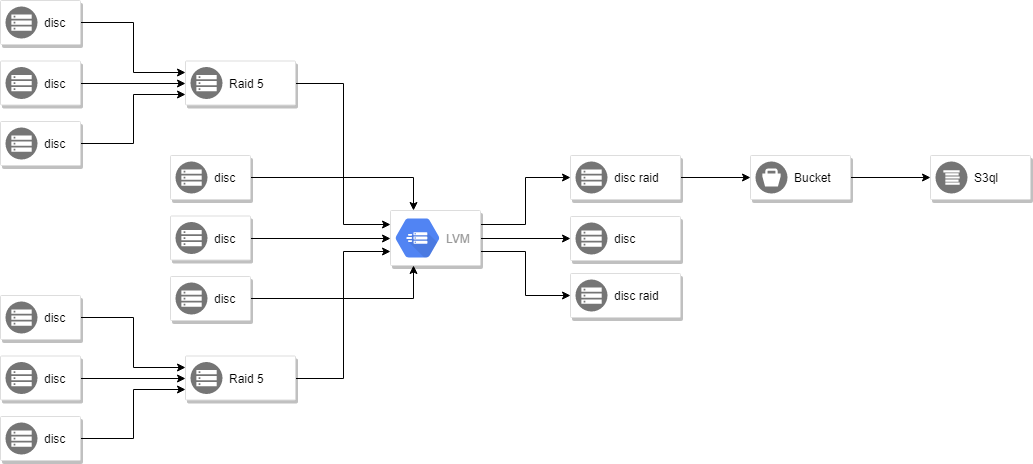
\includegraphics[width=\textwidth]{structure.png}

\section{En este ejercicio se realizará la configuración de la impresora que se encuentra asociada al servidor y a la cual pueden acceder diferentes usuarios. Instalar un servidor de impresión CUPS y configurarlo de forma tal que:
}



\clearpage

\clearpage
\section{bibliografia}
https://www.tecmint.com/create-raid-5-in-linux/ \smallskip

https://es.wikipedia.org/wiki/RAID\smallskip

https://getfedora.org/es/workstation/\smallskip

https://www.tecmint.com/extend-and-reduce-lvms-in-linux/\smallskip

https://www.draw.io\smallskip
\end{document}
